\documentclass[10pt, oneside, final]{article}
\usepackage{parskip}
\usepackage{graphicx}
\usepackage{hyperref}
\usepackage[
  paperwidth = 3.5in,
  paperheight = 2in,
  margin = 0.2in,
  noheadfoot
]{geometry}
\usepackage{wrapfig}
\usepackage[scaled = 0.9]{FiraSans}
\usepackage[varqu, scaled = 0.95]{zi4}
\usepackage{fontawesome} % icons

\setlength{\baselineskip}{0cm} % between baselines
\setlength{\topskip}{0pt}      % between header and text block

\begin{document}
  \thispagestyle{empty}
  \begin{wrapfigure}{r}{0.3\textwidth}
  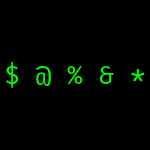
\includegraphics[width = 0.3\textwidth]{business_card.png}
  \end{wrapfigure}
  \underline{\large\textsf{\textbf{Elvin Aslanov}}}
  {Unix specialist} \\
  \\
  {\href{https://openbsd.org/}{OpenBSD}, \href{https://perl.org/}{Perl}, and \href{https://postgresql.org/}{PostgreSQL}} \\
  \\
  \emph{\href{https://en.wikipedia.org/wiki/Open-source_software}{open source software} development, deployment, and configuration}
  \vfill 
  {\faEnvelope} \texttt{\href{mailto:rwp.primary@gmail.com}{rwp.primary@gmail.com}} \hfill 
  {\faGithub} \texttt{\href{https://github.com/rwp0}{rwp0}} \\
  {\faPhone} \href{tel:+994702081512}{+994{\textendash}70{\textendash}208{\textendash}15{\textendash}12}
 \hfill
  {\faGlobe} \texttt{\href{https://rwp0.github.io/}{rwp0.github.io}} \\
  {\faCertificate} \texttt{\href{https://cs.lpi.org/caf/Xamman/certification/verify/LPI000307519/bafrejwgeb}{LPIC-2}, \href{https://cs.lpi.org/caf/Xamman/certification/verify/LPI000307519/mvuk2szhhw}{LPI-BSDS}}
\end{document}
